% --------------------------------------------------
% DOCUMENT CLASS
% --------------------------------------------------

\documentclass[
thesis.tex
]{subfiles}

\begin{document}

In this section, the model calibration is presented, along with the corresponding impulse response functions.

In due time, a thorough analysis of the results will be conducted.

Following that, a Bayesian estimation will be performed to estimate the model parameters.
	
	\subsection{Calibration}
	
	% --------------------------------------------------
	% PARAMETER CALIBRATION
	% --------------------------------------------------
	
	\subsubsection{Parameter Calibration}
	
	\vspace*{0.5cm}
	
	\begin{center}
		
		\begin{longtblr}[
			label = {table:parameter-calibration},
			caption = {Parameter Calibration},
			remark{Source} = {\cite{costa_junior_understanding_2016}},
			]{rowhead = 1,
				colspec = {
					Q[c]
					|Q[l]
					|Q[si={table-format=3.2,table-number-alignment=center},c,white]
				}
			}
			\hline[2pt]
			\textbf{Parameter} & \textbf{Definition} & \textbf{Calibration} \\ \hline[2pt]
			$\alpha$           & production elasticity with respect to capital & $0.35$ \\ \hline
			$\beta$            & intertemporal discount factor & $0.985$ \\ \hline
			$\gamma_R$         & interest-rate smoothing parameter & $0.79$ \\ \hline
			$\gamma_\pi$       & interest-rate sensitivity in relation to inflation & $2.43$ \\ \hline
			$\gamma_Y$         & interest-rate sensitivity in relation to product & $0.16$ \\ \hline
			$\delta$           & capital depreciation rate & $0.025$ \\ \hline
			$\theta$           & price stickness parameter & $0.8$ \\ \hline
			$\theta_C$         & consumption weight in production  & $0.8$ \\ \hline
			$\theta_I$         & investment weight in production  & $1 -\theta_C$ \\ \hline
			$\rho_A$           & autoregressive parameter of productivity & $0.95$ \\ \hline
			$\rho_M$           & autoregressive parameter of monetary policy & $0.9$ \\ \hline
			$\sigma$           & relative risk aversion coefficient & $2$ \\ \hline
			$\phi$             & relative labor weight in utility & $1$ \\ \hline
			$\varphi$          & marginal disutility of labor supply & $1.5$ \\ \hline
			$\psi$             & elasticity of substitution between intermediate goods & $8$ \\ \hline[2pt]
		\end{longtblr}
		
	\end{center}
	
% \newpage
	
	% --------------------------------------------------
	% VARIABLES AT THE STEADY STATE
	% --------------------------------------------------
	
	\subsubsection{Variables at the Steady State}
	
	\vspace*{0.5cm}
	
	\begin{center}
		
		\begin{longtblr}[
			label = {table:ss-values},
			caption = {Steady State Values},
			remark{Source} = {The author.},
			]{rowhead = 1,
				colspec = {
					Q[c]
					|Q[si={table-format=3.2,table-number-alignment=center},c,white]
				}
			}
			\hline[2pt]
			\textbf{Variable} & \textbf{Steady State Value} \\
			\hline[2pt]
			$P$               & $1$ \\
			\hline
			$Z_A$             & $1$ \\
			\hline
			$P^\ast$          & $1$ \\
			\hline
			$\pi$             & $1$ \\
			\hline
			$Z_M$             & $1$ \\
			\hline
			$R$               & $0.0402$ \\
			\hline
			$\Lambda$         & $0.8750$ \\
			\hline
			$W$               & $1.6967$ \\
			\hline
			$Y$               & $2.6366$ \\
			\hline
			$C$               & $2.1348$ \\
			\hline
			$I$               & $0.5018$ \\
			\hline
			$K$               & $20.0716$ \\
			\hline
			$L$               & $0.8838$ \\
			\hline[2pt]
		\end{longtblr}
		
	\end{center}
	
% \newpage

%%%%%%%%%%%%%%%%%%%%%%%%%%%%%%%%%%%%%%%%%%%%%%%%%%%%%%%%

%% --------------------------------------------------
%% PARAMETER CALIBRATION
%% --------------------------------------------------
%
%\subsubsection{Parameter Calibration}
%
%\vspace*{-1cm}
%
%\begin{center}
%	
%	\begin{align}
%		\begin{bmatrix}
%			\phi       \\
%			\varphi    \\
%			\sigma     \\
%			\beta      \\
%			\delta     \\
%			\psi       \\
%			\theta     \\
%			\alpha     \\
%			\gamma_R   \\
%			\gamma_\pi \\
%			\gamma_Y   \\
%			\rho_A     \\
%			\rho_M     \\
%			\theta_C   \\
%			\theta_I
%		\end{bmatrix} = 
%		\begin{bmatrix}
%			\phi       \\
%			\varphi    \\
%			\sigma     \\
%			\beta      \\
%			\delta     \\
%			\psi       \\
%			\theta     \\
%			\alpha     \\
%			\gamma_R   \\
%			\gamma_\pi \\
%			\gamma_Y   \\
%			\rho_A     \\
%			\rho_M     \\
%			\theta_C   \\
%			\theta_I   
%		\end{bmatrix}
%	\end{align}
%	
%\end{center}
%
%% --------------------------------------------------
%% VARIABLES AT THE STEADY STATE
%% --------------------------------------------------
%
%\subsubsection{Variables at the Steady State}
%
%\vspace*{-1cm}
%
%\begin{align}
%	\begin{bmatrix}
%		P \\
%		Z_A \\
%		P^\ast \\
%		\pi \\
%		Z_M \\
%		R \\
%		\Lambda \\
%		W \\
%		Y \\
%		C \\
%		I \\
%		K \\
%		L
%	\end{bmatrix} = 
%	\begin{bmatrix}
%		P \\
%		Z_A \\
%		P^\ast \\
%		\pi \\
%		Z_M \\
%		R \\
%		\Lambda \\
%		W \\
%		Y \\
%		C \\
%		I \\
%		K \\
%		L
%	\end{bmatrix}
%\end{align}
%
%\newpage

%%%%%%%%%%%%%%%%%%%%%%%%%%%%%%%%%%%%%%%%%%%%%%%%%%%%%%%%
	
	% --------------------------------------------------
	% IMPULSE RESPONSE GRAPHICS
	% --------------------------------------------------
	
	\subsection{Impulse Response Functions}
	
	These are the impulse response functions of model in section \ref{sec:model}. In due time, the IRF of section \ref{sec:regional-model} will be presented.
	
	\subsubsection{Productivity Shock}
	
	\begin{figure}[h!]
		\centering
		\begin{subfigure}[b]{0.3\textwidth}
			\centering
			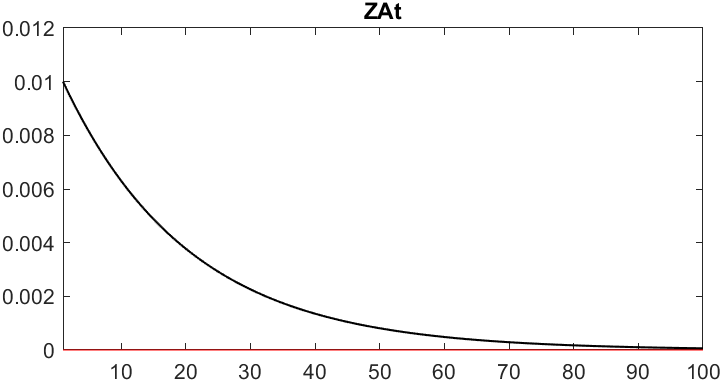
\includegraphics[width=\textwidth]{shock_ZAt/shock_ZAt_ZAt}
			\caption{Productivity Shock}
			\label{fig:zat-productivity-shock}
		\end{subfigure}
		\hfill
		\begin{subfigure}[b]{0.3\textwidth}
			\centering
			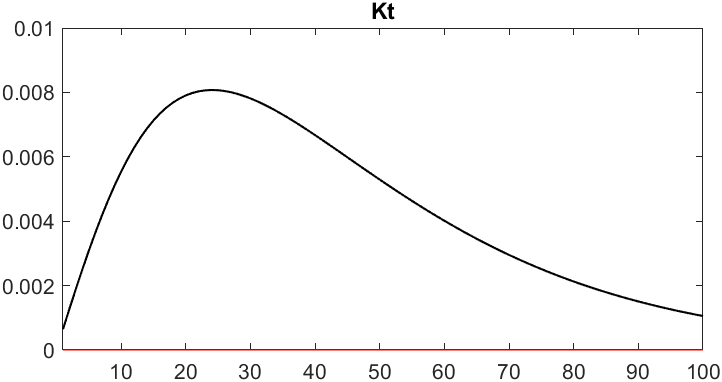
\includegraphics[width=\textwidth]{shock_ZAt/shock_ZAt_Kt}
			\caption{Capital}
			\label{fig:zat-capital}
		\end{subfigure}
		\hfill
		\begin{subfigure}[b]{0.3\textwidth}
			\centering
			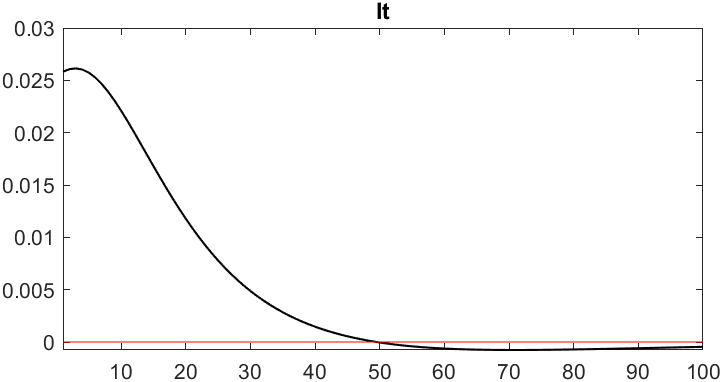
\includegraphics[width=\textwidth]{shock_ZAt/shock_ZAt_It}
			\caption{Investment}
			\label{fig:zat-investment}
		\end{subfigure}
		\hfill
		
		\vspace*{0.5cm}
		
		\begin{subfigure}[b]{0.3\textwidth}
			\centering
			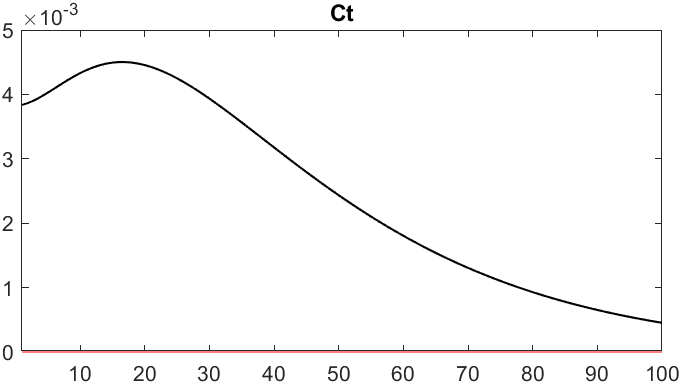
\includegraphics[width=\textwidth]{shock_ZAt/shock_ZAt_Ct}
			\caption{Consumption}
			\label{fig:zat-consumption}
		\end{subfigure}
		\hfill
		\begin{subfigure}[b]{0.3\textwidth}
			\centering
			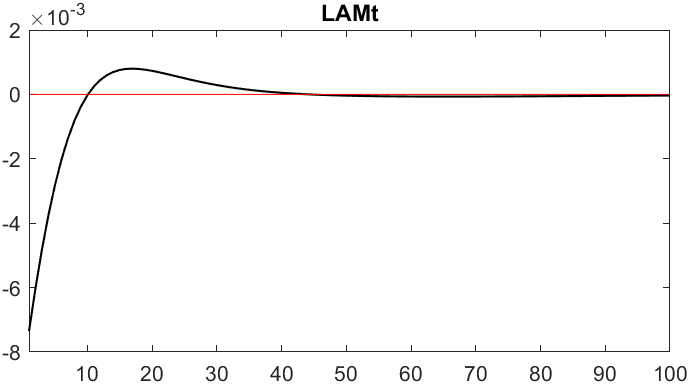
\includegraphics[width=\textwidth]{shock_ZAt/shock_ZAt_LAMBDAt}
			\caption{Marginal Cost}
			\label{fig:zat-marginal-cost}
		\end{subfigure}
		\hfill
		\begin{subfigure}[b]{0.3\textwidth}
			\centering
			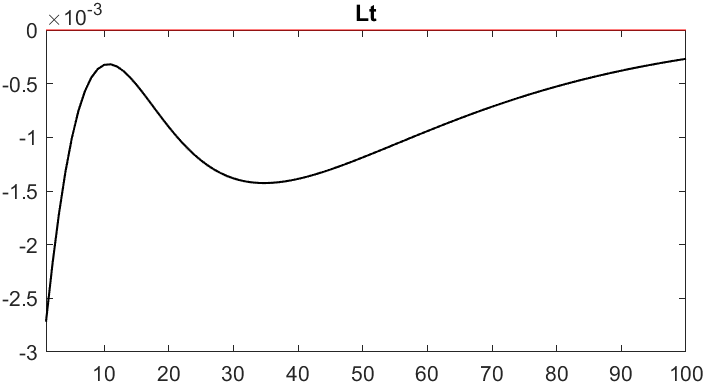
\includegraphics[width=\textwidth]{shock_ZAt/shock_ZAt_Lt}
			\caption{Labor}
			\label{fig:zat-labor}
		\end{subfigure}
		\hfill
		
		\vspace*{0.5cm}
		
		\begin{subfigure}[b]{0.3\textwidth}
			\centering
			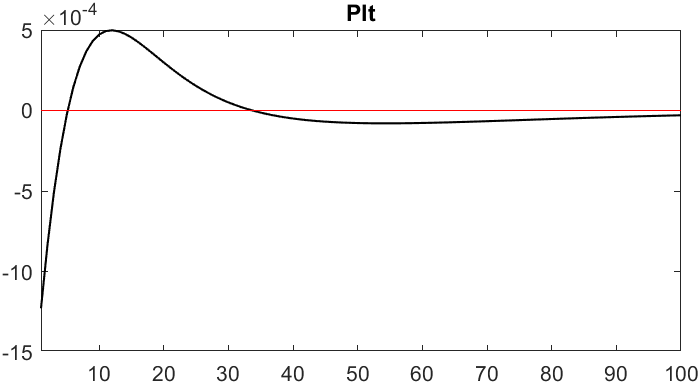
\includegraphics[width=\textwidth]{shock_ZAt/shock_ZAt_PIt}
			\caption{Inflation}
			\label{fig:zat-inflation}
		\end{subfigure}
		\hfill
		\begin{subfigure}[b]{0.3\textwidth}
			\centering
			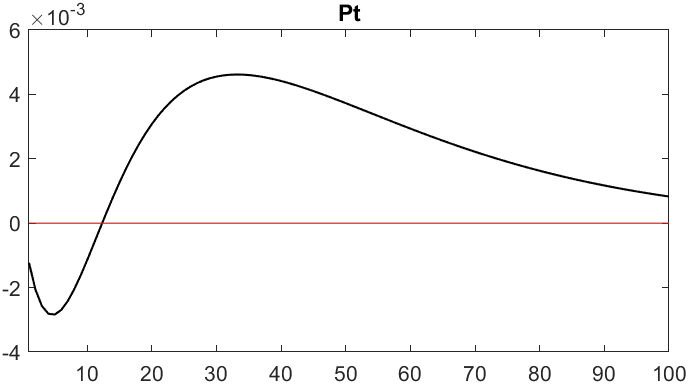
\includegraphics[width=\textwidth]{shock_ZAt/shock_ZAt_Pt}
			\caption{Price Level}
			\label{fig:zat-price}
		\end{subfigure}
		\hfill
		\begin{subfigure}[b]{0.3\textwidth}
			\centering
			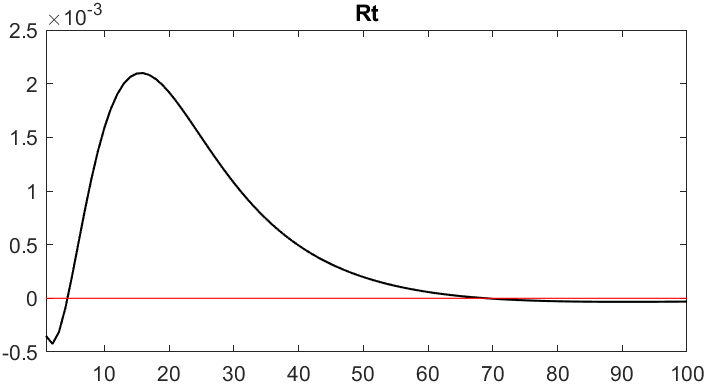
\includegraphics[width=\textwidth]{shock_ZAt/shock_ZAt_Rt}
			\caption{Interest Rate}
			\label{fig:zat-interest-rate}
		\end{subfigure}
		\hfill
		
		\vspace*{0.5cm}
		
		\begin{subfigure}[b]{0.3\textwidth}
			\centering
			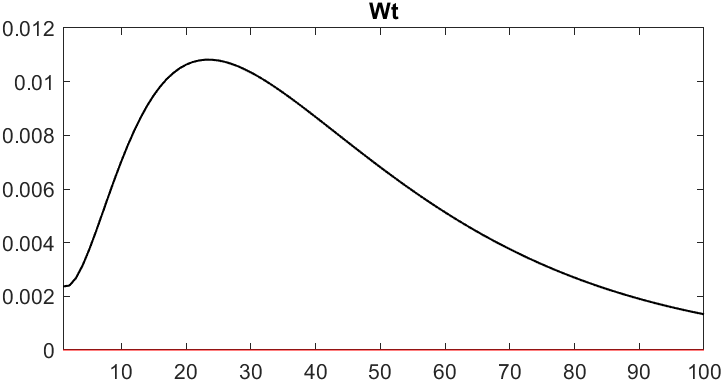
\includegraphics[width=\textwidth]{shock_ZAt/shock_ZAt_Wt}
			\caption{Wage}
			\label{fig:zat-wage}
		\end{subfigure}
		\hfill
		\begin{subfigure}[b]{0.3\textwidth}
			\centering
			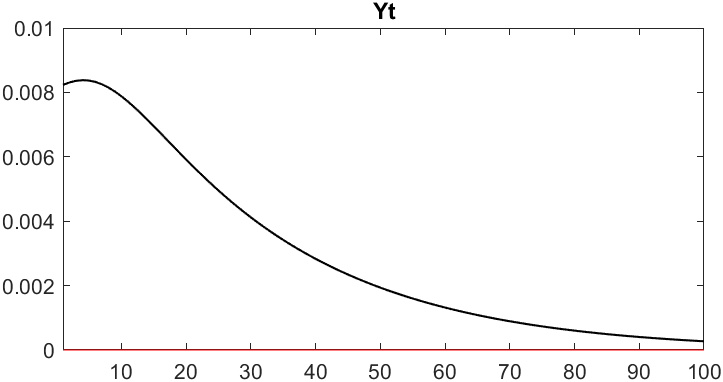
\includegraphics[width=\textwidth]{shock_ZAt/shock_ZAt_Yt}
			\caption{Production}
			\label{fig:zat-production}
		\end{subfigure}
		\hfill
		\begin{subfigure}[b]{0.3\textwidth}
			\centering
			
\includegraphics[width=\textwidth]{shock_ZAt/blank}
		\end{subfigure}
		\hfill
		\caption{Productivity Shock Impulse Response Functions}
		\label{fig:zat-irf}
	\end{figure}
	
	\newpage
	
	\subsubsection{Monetary Shock}
	
	\begin{figure}[h!]
		\centering
		\begin{subfigure}[b]{0.3\textwidth}
			\centering
			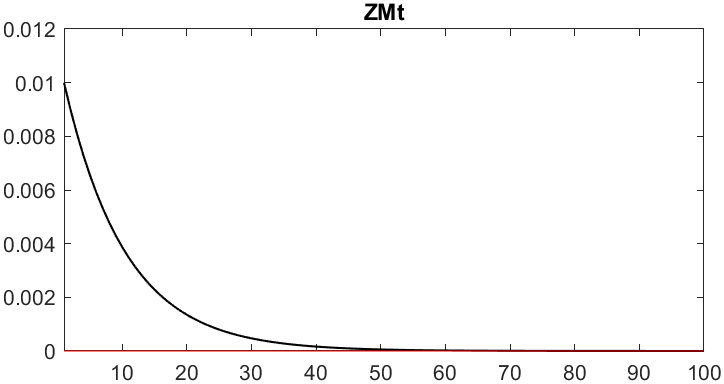
\includegraphics[width=\textwidth]{shock_ZMt/shock_ZMt_ZMt}
			\caption{Monetary Shock}
			\label{fig:ZMt-monetary-shock}
		\end{subfigure}
		\hfill
		\begin{subfigure}[b]{0.3\textwidth}
			\centering
			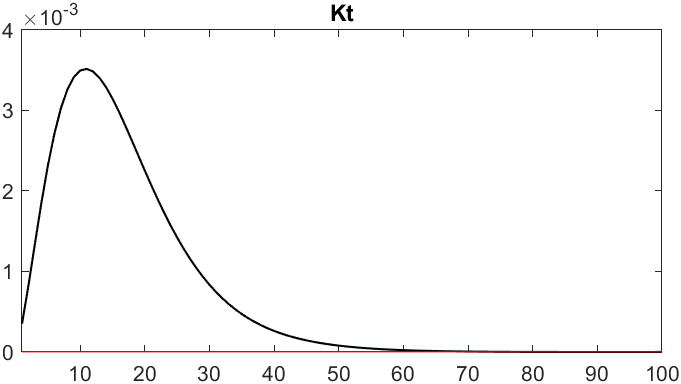
\includegraphics[width=\textwidth]{shock_ZMt/shock_ZMt_Kt}
			\caption{Capital}
			\label{fig:ZMt-capital}
		\end{subfigure}
		\hfill
		\begin{subfigure}[b]{0.3\textwidth}
			\centering
			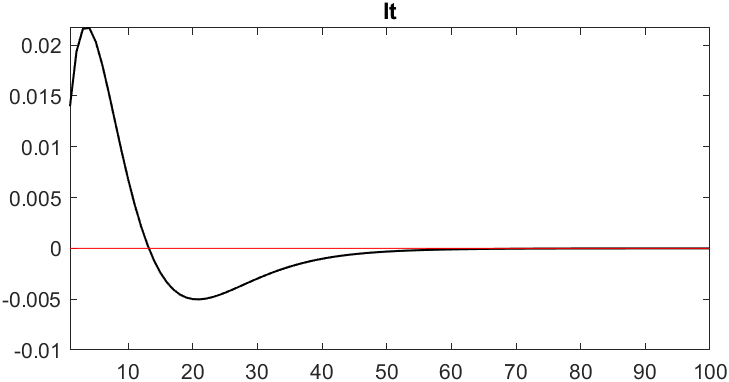
\includegraphics[width=\textwidth]{shock_ZMt/shock_ZMt_It}
			\caption{Investment}
			\label{fig:ZMt-investment}
		\end{subfigure}
		\hfill
		
		\vspace*{0.5cm}
		
		\begin{subfigure}[b]{0.3\textwidth}
			\centering
			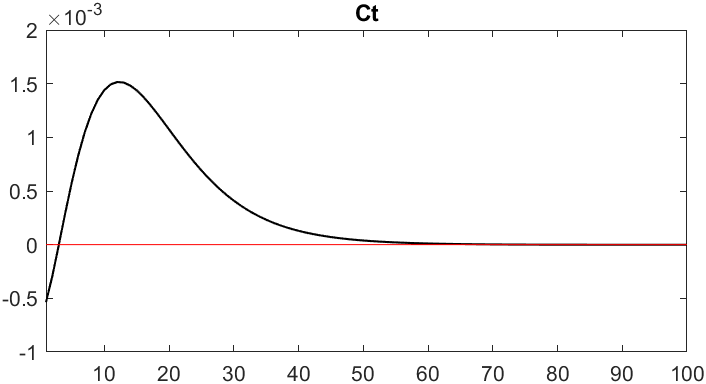
\includegraphics[width=\textwidth]{shock_ZMt/shock_ZMt_Ct}
			\caption{Consumption}
			\label{fig:ZMt-consumption}
		\end{subfigure}
		\hfill
		\begin{subfigure}[b]{0.3\textwidth}
			\centering
			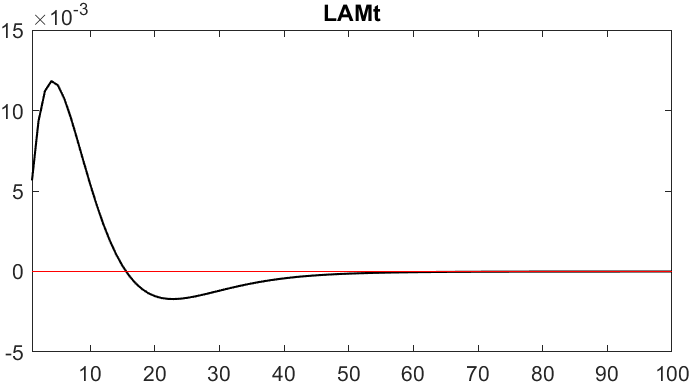
\includegraphics[width=\textwidth]{shock_ZMt/shock_ZMt_LAMBDAt}
			\caption{Marginal Cost}
			\label{fig:ZMt-marginal-cost}
		\end{subfigure}
		\hfill
		\begin{subfigure}[b]{0.3\textwidth}
			\centering
			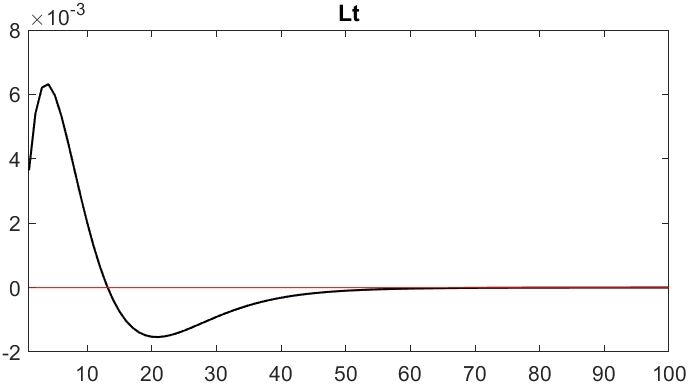
\includegraphics[width=\textwidth]{shock_ZMt/shock_ZMt_Lt}
			\caption{Labor}
			\label{fig:ZMt-labor}
		\end{subfigure}
		\hfill
		
		\vspace*{0.5cm}
		
		\begin{subfigure}[b]{0.3\textwidth}
			\centering
			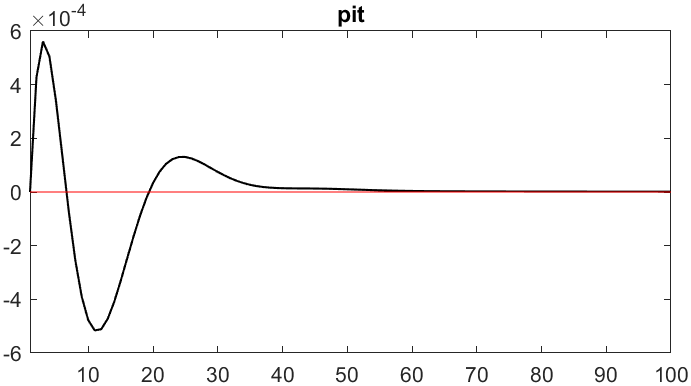
\includegraphics[width=\textwidth]{shock_ZMt/shock_ZMt_PIt}
			\caption{Inflation}
			\label{fig:ZMt-inflation}
		\end{subfigure}
		\hfill
		\begin{subfigure}[b]{0.3\textwidth}
			\centering
			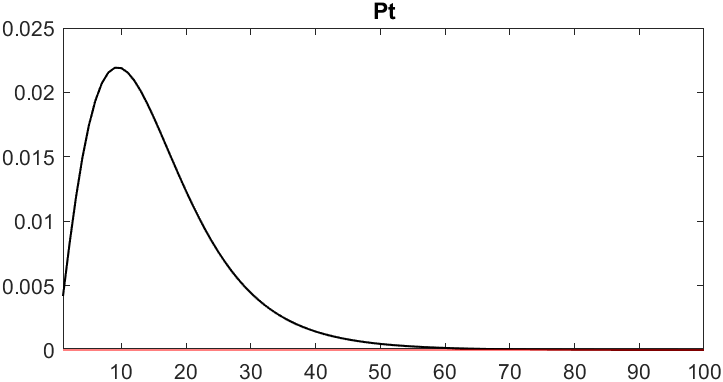
\includegraphics[width=\textwidth]{shock_ZMt/shock_ZMt_Pt}
			\caption{Price Level}
			\label{fig:ZMt-price}
		\end{subfigure}
		\hfill
		\begin{subfigure}[b]{0.3\textwidth}
			\centering
			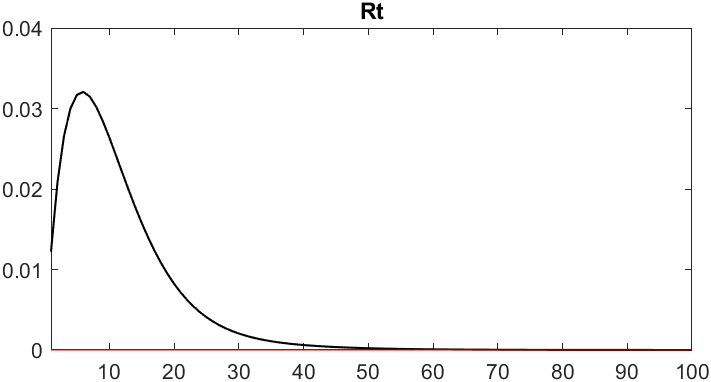
\includegraphics[width=\textwidth]{shock_ZMt/shock_ZMt_Rt}
			\caption{Interest Rate}
			\label{fig:ZMt-interest-rate}
		\end{subfigure}
		\hfill
		
		\vspace*{0.5cm}
		
		\begin{subfigure}[b]{0.3\textwidth}
			\centering
			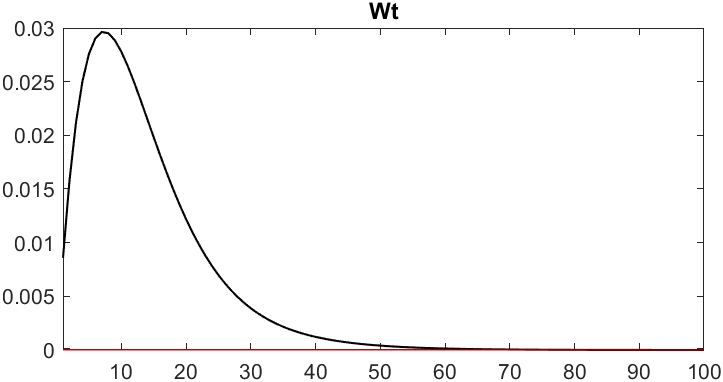
\includegraphics[width=\textwidth]{shock_ZMt/shock_ZMt_Wt}
			\caption{Wage}
			\label{fig:ZMt-wage}
		\end{subfigure}
		\hfill
		\begin{subfigure}[b]{0.3\textwidth}
			\centering
			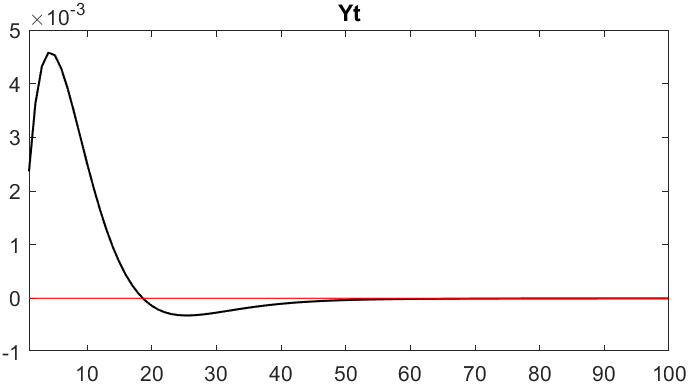
\includegraphics[width=\textwidth]{shock_ZMt/shock_ZMt_Yt}
			\caption{Production}
			\label{fig:ZMt-production}
		\end{subfigure}
		\hfill
		\begin{subfigure}[b]{0.3\textwidth}
			\centering
			
\includegraphics[width=\textwidth]{shock_ZMt/blank}
		\end{subfigure}
		\hfill
		\caption{Monetary Shock Impulse Response Functions}
		\label{fig:ZMt-irf}
	\end{figure}
	
	\newpage
	
	\subsection{Parametrization}
	
	To be done.

\end{document}